\chapter{Firebase}

Das nächste Kapitel beschreibt die Architektur und die Implementierung der geplanten Anwendung mit Google Firebase.

\section{Architektur}

Für die Architektur wird zunächst die Lösungsstrategie vorgestellt. Darauf folgen die Bausteinsicht, die Laufzeitsicht sowie die Verteilungssicht.

\subsection{Lösungsstrategie}

Ebenfalls wie bei \ac{AWS} Amplify lässt sich die Architektur von Firebase in Präsentation, Logik und Datenhaltung aufteilen, welche durch unterschiedliche Cloud-Dienste und Frameworks abgebildet sind.
\begin{itemize}
  \item Präsentation
    \begin{itemize}
      \item React.js mit TypeScript
      \item Firebase Javascript SDK
    \end{itemize}
  \item Logik
    \begin{itemize}
      \item Authentication
      \item Cloud Functions
      \item Transcoder API
      \item IAM
    \end{itemize}
  \item Datenhaltung
    \begin{itemize}
      \item Authentication
      \item Cloud Firestore
      \item Cloud Storage
      \item IAM
      \item Firebase Hosting
    \end{itemize}
\end{itemize}

Die Dienste IAM und Authentication befindet sich zugleich in der Logik als auch in der Datenhaltung, da dort neben der Authentifizierung und Autorisierung auch die Benutzer persistiert werden.

Auch hier werden ausschließlich interne Dienste der Google Cloud verwendet, so dass die Rahmenbedingungen nicht missachtet sind und die beiden Technologien vergleichbar sind. Abgesehen von Cloud-Diensten ist der Unterschied beider Projekte auf technischer Ebene, dass die Firebase-Anwendung im Backend TypeScript statt JavaScript verwendet.

Als nächstes werden Lösungsansätze, um die nichtfunktionalen Anforderungen, auch Qualitätsziele genannt, zu erreichen:

<<<<<todo
\begin{description}
   \item[Verfügbarkeit] Firebase bietet für Frontend und Backend ein Zero-Downtime Deployment.
   \item[Skalierbarkeit] Durch die Serverless-Architektur skalieren Funktionen sowie Firestore automatisch innerhalb der \ac{Google}-Cloud.
   \item[Analysierbarkeit] Durch den Einsatz von Cloud Logging können Anfragen für Funktionen nachvollzogen werden.
   \item[Interoperabilität] Es wird keine REST- oder GraphQL-Schnittstelle genutzt. Stattdessen werden die Funktionen des Backends direkt aufgerufen. Damit ist die Interoperabilität nicht direkt gegeben.
   \item[Backups] Backups lassen sich automatisiert über Firestore aktivieren.
   \item[Wiederherstellbarkeit] Das Backup von Firestore muss manuell eingespielt werden..
\end{description}
<<<< todo end

\subsection{Bausteinsicht}

\subsection{Laufzeitsicht}

\subsubsection{Auflisten, Aktualisieren und Löschen eines Videos}

\begin{figure}
  \centering
  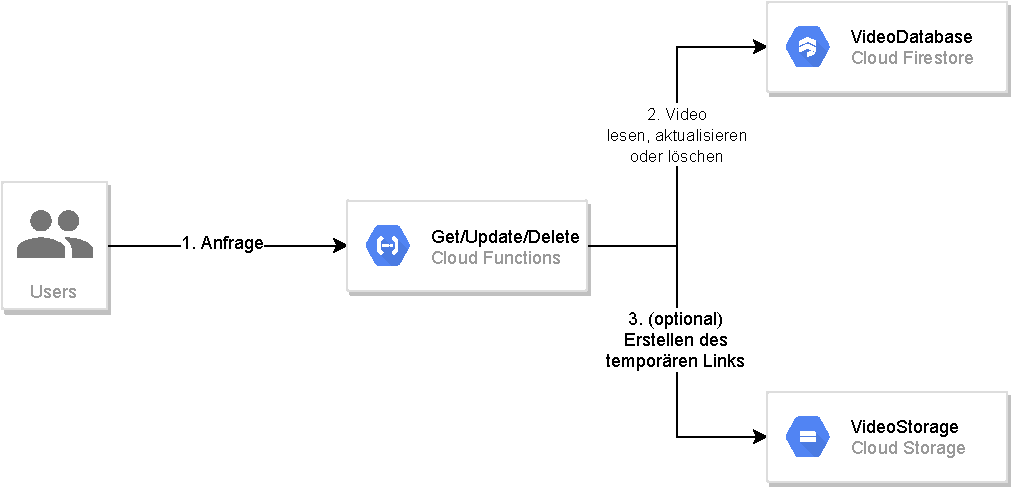
\includegraphics[width=1\columnwidth]{6_firebase/laufzeitsicht_1.pdf}
  \caption{Firebase - Laufzeitsicht - Lesen, Aktualisieren und Löschen eines Videos}
  \label{Firebase:laufzeitsicht1}
\end{figure}


Ablauf:
- Functions: update, delete
- 1. Call auf Function
- 2. Call auf Firestore von Function

- 3. Call auf Firebase Storage für presignedLink

- Besonderheiten beim Lesen
  - Search

- Besonderheiten bei Permissions (?)
  - prüfen, ob admin rolle oder ob owner, aber alles in separater DB gespeichert, nicht wie bei Cognito

\subsubsection{Erstellen eines Videos}

\begin{figure}
  \centering
  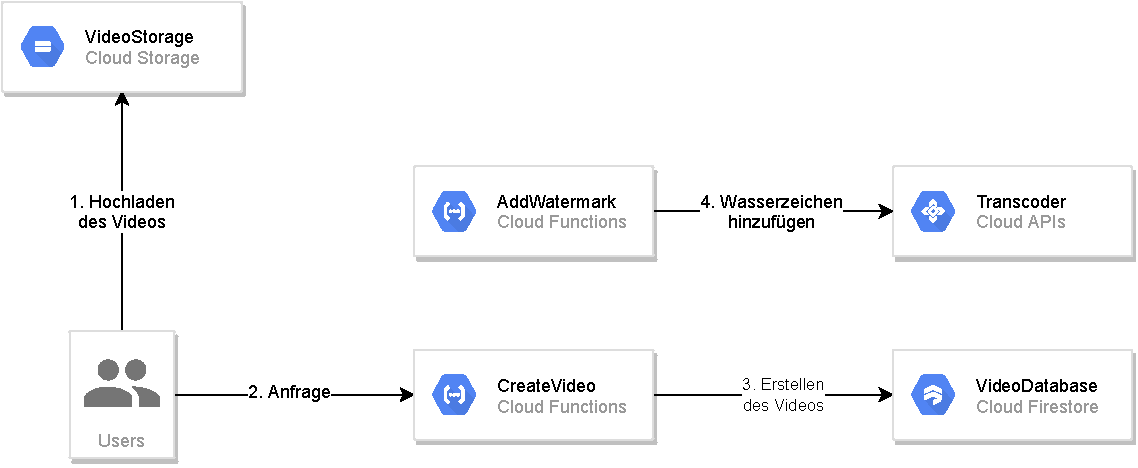
\includegraphics[width=1\columnwidth]{6_firebase/laufzeitsicht_2.pdf}
  \caption{Firebase - Laufzeitsicht - Erstellen eines Videos}
  \label{Firebase:laufzeitsicht2}
\end{figure}

Functions:
- AddWaterMarkToVideo
- createVideo

0. Upload in firestore storage
1. Call to createVideo
2. Create video in firebase (with raw link to firestore)
3. Firestore Trigger executes on Create video/{docId}
4. Calls video-transcoder to add watermark, put in storage and put the new link in Firestore again


\subsection{Verteilungssicht}

\section{Implementierung}

todo